\documentclass[aspectratio=169,11pt]{beamer}
\usepackage{azzurri}
\usepackage{graphicx}
\usepackage{booktabs}
\usepackage{colortbl}
\graphicspath{{../output/figures/}}

\title{Prevention Without Proof}
\subtitle{Did national suicide-prevention strategies reduce suicide?}
\author{Scott Cunningham}
\institute{Baylor University}
\date{European Commission \,\textperiodcentered\, Joint Research Centre, Ispra \,\textperiodcentered\, June 2026}

\begin{document}

% ---------- Act I ----------
\begin{frame}[plain]\titlepage\end{frame}

\bignumber{40s}{Somewhere on earth, about every forty seconds, a person decides the rest of life is not worth the rest of life.}

\begin{frame}{More than war, more than homicide}
\begin{columns}[T]
\begin{column}{0.55\textwidth}
\vspace{1.2em}
{\Large More than \textbf{700{,}000} suicides a year.}\\[1.2em]
{\large More than war.}\\[0.4em]
{\large More than homicide.}\\[0.4em]
{\large More than most diseases we built ministries to defeat.}
\end{column}
\begin{column}{0.42\textwidth}
\vspace{0.6em}
\begin{block}{The number is stubborn}
It has barely moved in a generation.
\end{block}
\end{column}
\end{columns}
\end{frame}

\begin{frame}{The world answered with a document}
\begin{columns}[T]
\begin{column}{0.6\textwidth}
\vspace{0.8em}
\textbf{Finland}, 1986--92: investigate every suicide, build a national program.\\[0.8em]
Then everyone copied it: Norway and Sweden 1995, France 2000, the UK 2002, Ireland 2005.\\[0.8em]
By 2018 the WHO urges \emph{every} member state to adopt one.
\end{column}
\begin{column}{0.38\textwidth}
\vspace{1.4em}
\begin{alertblock}{The premise}
We decided, collectively, that the \textbf{strategy document} is the cure.
\end{alertblock}
\end{column}
\end{columns}
\end{frame}

\begin{frame}{The only question that matters}
\vfill
\begin{center}
{\Large Does a country that adopts a national strategy}\\[0.5em]
{\Large bury \textbf{fewer} of its citizens than it otherwise would have?}
\end{center}
\vfill
\begin{center}\color{warmgray}Empirical. Answerable in principle. Almost entirely unanswered in practice.\end{center}
\vfill
\end{frame}

\begin{frame}{My answer, stated up front}
\vfill
\begin{center}
{\Large From the cross-national record, \textbf{we cannot tell}}\\[0.6em]
{\Large whether these strategies have saved a single life.}
\end{center}
\vfill
\begin{center}\color{tricrosso}\large That should frighten the skeptic and the believer alike.\end{center}
\vfill
\end{frame}

% ---------- Act II ----------
\divider{The famous answer}{And the method underneath it}

\begin{frame}{The canonical finding looked protective}
\begin{columns}[T]
\begin{column}{0.6\textwidth}
\vspace{1em}
Matsubayashi \& Ueda (2011): across 21 OECD countries, those with national programs saw suicide \textbf{fall} relative to those without.\\[1em]
It became the evidence base for a global policy.
\end{column}
\begin{column}{0.38\textwidth}
\vspace{1.2em}
\begin{block}{The engine}
A two-way fixed-effects comparison of adopters vs.\ non-adopters.
\end{block}
\end{column}
\end{columns}
\end{frame}

\begin{frame}{Two-way fixed effects misleads under staggered timing}
\vspace{0.6em}
When units adopt at different dates and effects are heterogeneous, TWFE uses \textbf{already-treated units as controls} for newly-treated ones.
\begin{itemize}
\item The weights can be negative.
\item The estimate can fall outside the range of every true effect.
\item It can return the \textbf{wrong sign} for mechanical reasons.
\end{itemize}
\vspace{0.4em}
\begin{center}\color{warmgray}Goodman-Bacon (2021); de Chaisemartin \& D'Haultf\oe uille (2020).\end{center}
\end{frame}

\divider{The data}{All real --- nothing simulated}

\begin{frame}{Three real sources, one country-year panel}
\begin{itemize}
\item \textbf{Outcome:} Eurostat age-standardised suicide rate (ICD-10 X60--X84, Y87.0), 1994--2010.
\item \textbf{Treatment:} year a government adopted a stand-alone national strategy (WHO 2018; Lewitzka et al.\ 2019).
\item \textbf{Covariate:} World Bank unemployment --- the business cycle.
\end{itemize}
\vspace{0.5em}
\begin{center}\color{warmgray}Verified independently in R, Python, and Stata: identical samples and means.\end{center}
\end{frame}

\begin{frame}{The natural experiment is staggered --- and thin}
\centering
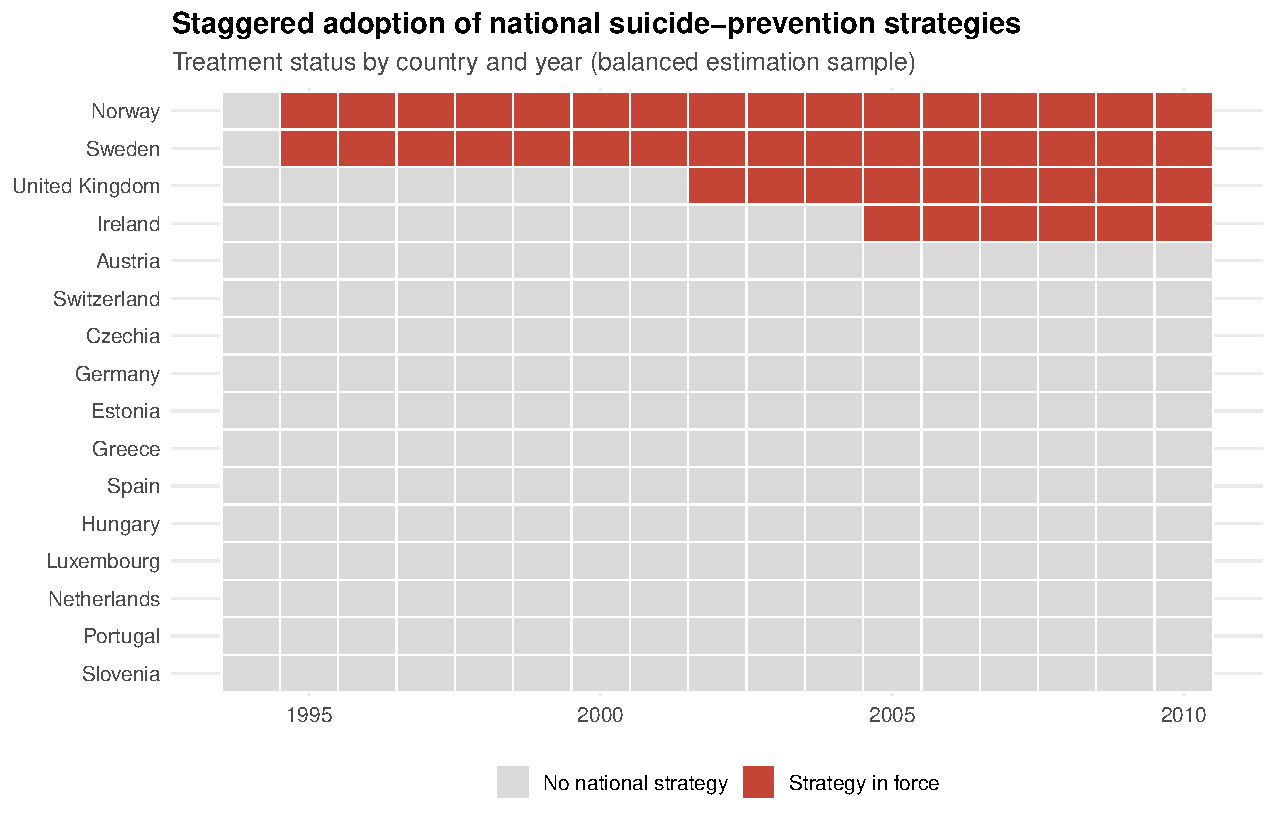
\includegraphics[height=0.73\textheight]{fig4_panelview.pdf}
\end{frame}

\begin{frame}{Four treated countries --- I will not pretend otherwise}
\centering
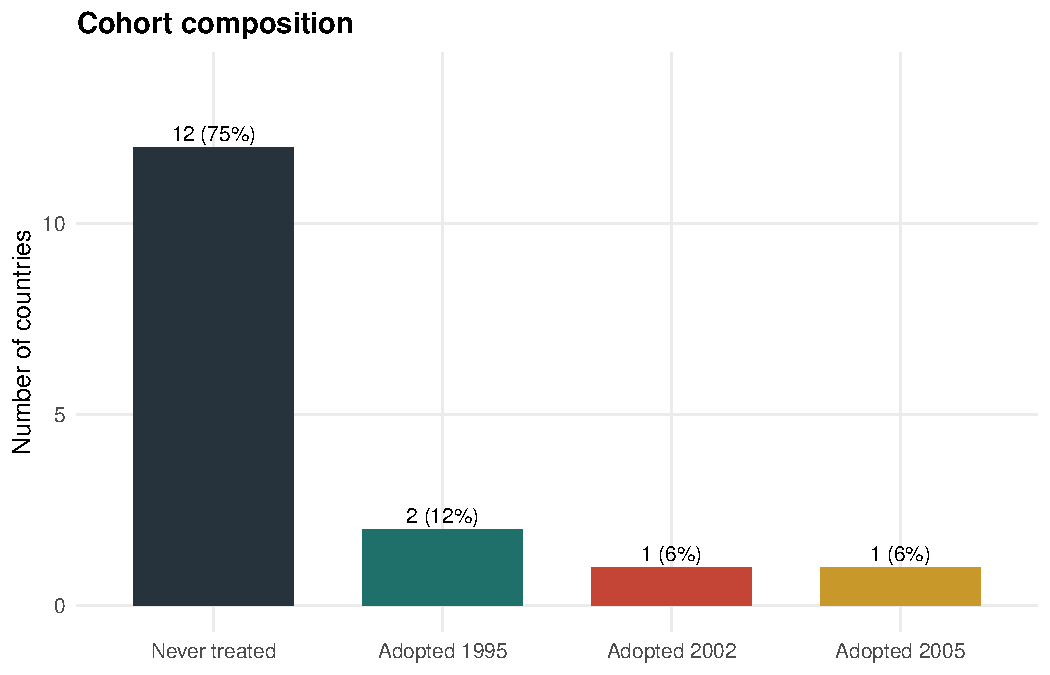
\includegraphics[height=0.74\textheight]{fig5_cohort_counts.pdf}
\end{frame}

\begin{frame}{Treated countries start lower; all bend up in the recession}
\centering
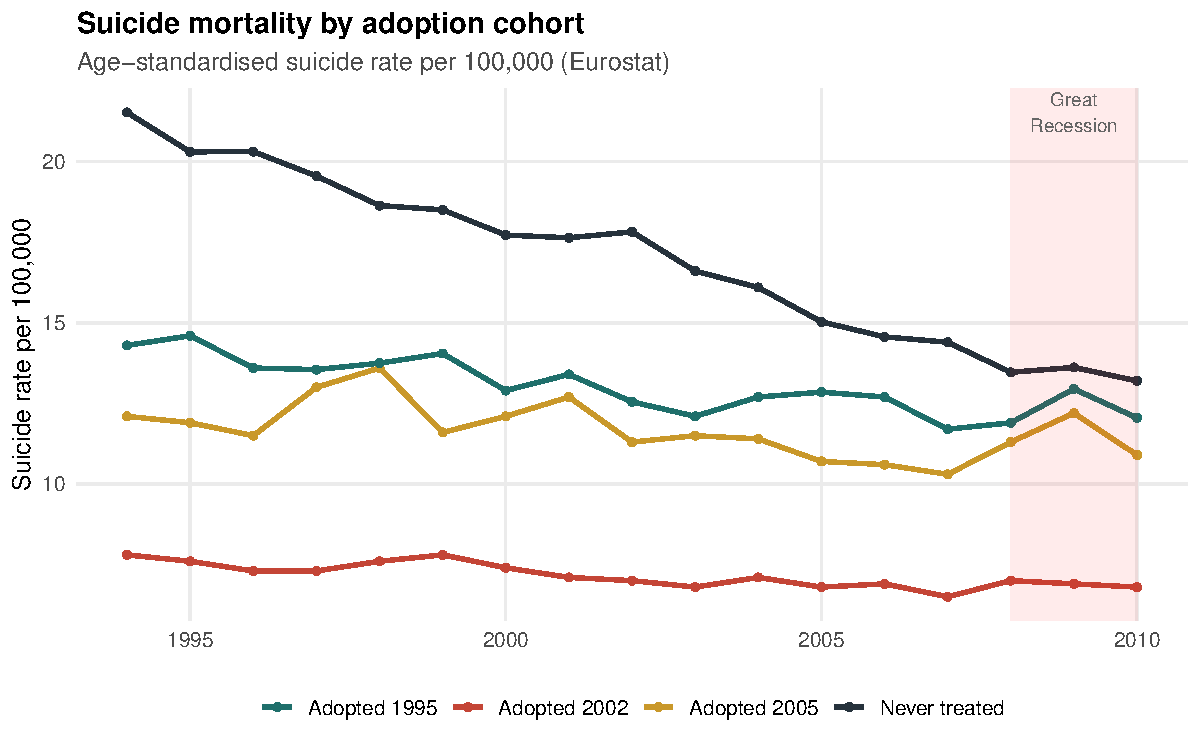
\includegraphics[height=0.73\textheight]{fig6_outcome_by_cohort.pdf}
\end{frame}

\divider{The design}{What we are trying to measure}

\begin{frame}{The estimand: a weighted average effect on the treated}
\vspace{0.8em}
For each adoption cohort $g$ and year $t$, compare the change in suicide against not-yet- and never-treated countries; aggregate, weighting cohorts by size.
\[
\theta = \sum_g w_g\,\overline{ATT}(g), \qquad w_g \propto \#\text{treated countries in } g.
\]
\vspace{0.3em}
\begin{center}\color{warmgray}Callaway \& Sant'Anna (2021), under \emph{conditional} parallel trends.\end{center}
\end{frame}

\begin{frame}{The covariate an expert would insist on}
\vfill
\begin{center}
{\Large Recessions raise suicide. Recoveries lower it.}\\[0.6em]
{\Large And Europe's recessions are not independent of its strategies.}
\end{center}
\vfill
\begin{center}\color{warmgray}So we condition on \textbf{unemployment} --- the fast-moving confounder that can wear a policy's clothes (Ruhm 2000; Reeves et al.\ 2012).\end{center}
\vfill
\end{frame}

\begin{frame}{And unemployment is genuinely imbalanced}
\vspace{0.6em}
\centering
\begin{tabular}{lccc}
\toprule
Baseline (1994) & Treated & Control & Std.\ diff. \\
\midrule
Suicide rate (per 100k) & 12.1 & 21.5 & $-0.99$ \\
\rowcolor{lightbg} Unemployment (\%) & 9.8 & 8.2 & $+0.33$ \\
Share aged 65+ (\%) & 15.2 & 14.0 & $+0.63$ \\
Median age (years) & 35.2 & 36.2 & $-0.42$ \\
\bottomrule
\end{tabular}
\vspace{0.8em}
\begin{center}\color{warmgray}Imbens \& Rubin (2015): $|\text{std.\ diff}| > 0.25$ is imbalanced. Unemployment clears it --- conditioning is necessary, not cosmetic.\end{center}
\end{frame}

\begin{frame}{There is no common support to weight on}
\centering
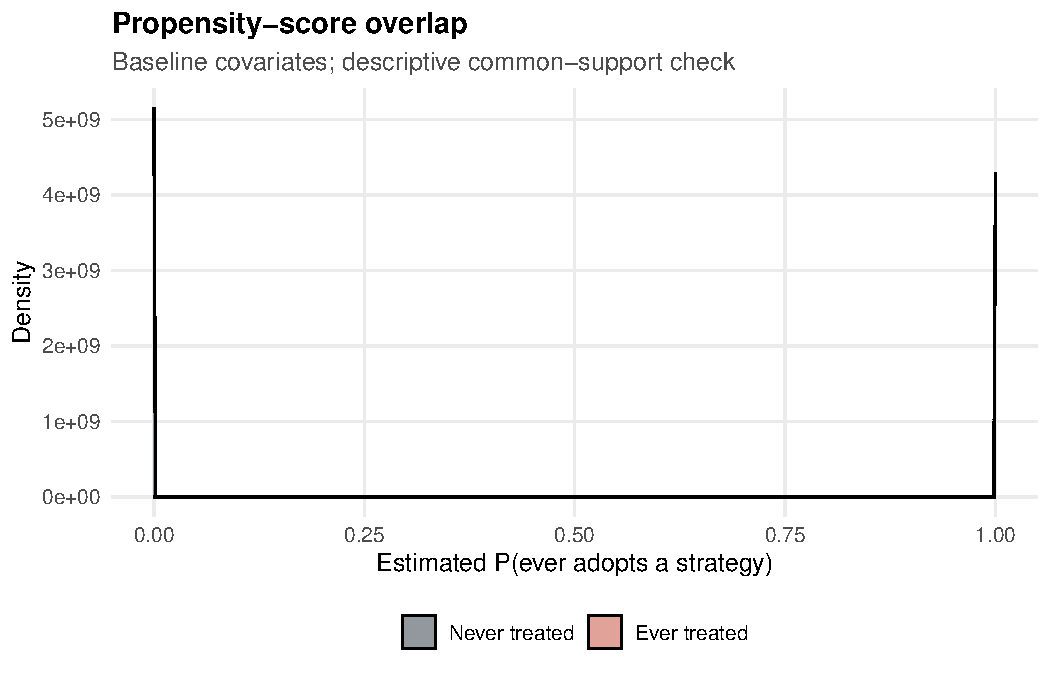
\includegraphics[height=0.66\textheight]{fig3_pscore_overlap.pdf}\\
{\color{warmgray}\small Perfect separation $\Rightarrow$ regression adjustment, not inverse-propensity weighting.}
\end{frame}

\begin{frame}{Sixteen clusters: trust the placebo, not the $t$-statistic}
\vspace{0.8em}
Four treated countries, twelve controls $\approx$ sixteen clusters.\\[0.6em]
Cluster-robust and bootstrap standard errors need many-cluster asymptotics this design does not have.
\begin{alertblock}{So the inferential weight is carried by randomization inference}
How often does \emph{fake} adoption, assigned at random among the never-treated, produce an estimate this large?
\end{alertblock}
\end{frame}

\divider{What the data say}{The inconvenient sign}

\begin{frame}{The estimate is positive: more suicide after adoption}
\vfill
\begin{center}
{\fontsize{52}{52}\selectfont\bfseries\color{tricrosso}$+2.7$}\\[0.8em]
{\Large suicides per 100{,}000, after adoption (s.e.\ 1.05)}
\end{center}
\vfill
\begin{center}\color{warmgray}Group-size-weighted ATT, Callaway--Sant'Anna, conditioning on unemployment.\end{center}
\vfill
\end{frame}

\begin{frame}{Three heterogeneity-robust estimators agree}
\centering
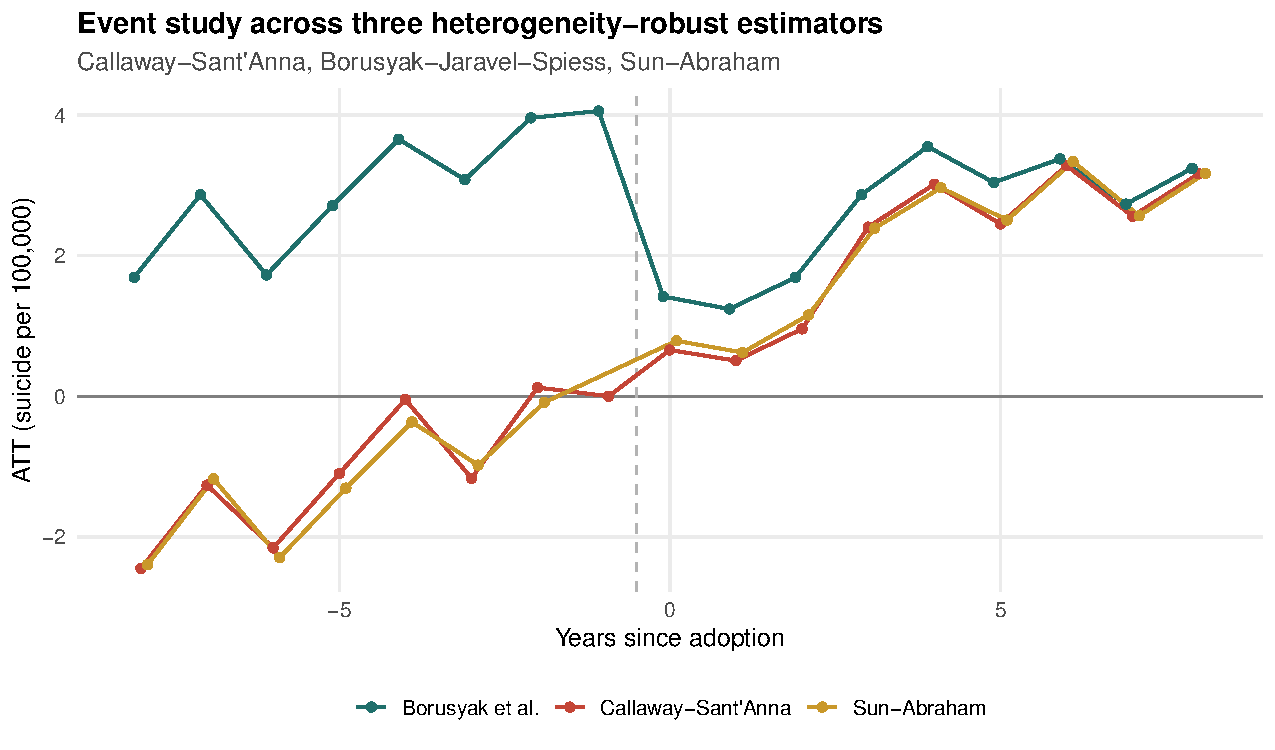
\includegraphics[height=0.62\textheight]{fig_robust_overlay.pdf}\\
{\color{warmgray}\small Callaway--Sant'Anna $+2.7$ \,\textperiodcentered\, Borusyak et al.\ $+3.2$ \,\textperiodcentered\, Sun--Abraham $+3.0$.}
\end{frame}

\begin{frame}{A careless reader would stop here}
\vfill
\begin{center}
{\Large ``Suicide-prevention strategies are followed by \emph{more} suicide.''}
\end{center}
\vfill
\begin{center}\color{tricrosso}\large Do not stop here.\end{center}
\vfill
\end{frame}

\divider{What the number is \emph{not}}{Five windows, one answer}

\begin{frame}{Measured correctly, pre-trends are flat}
\centering
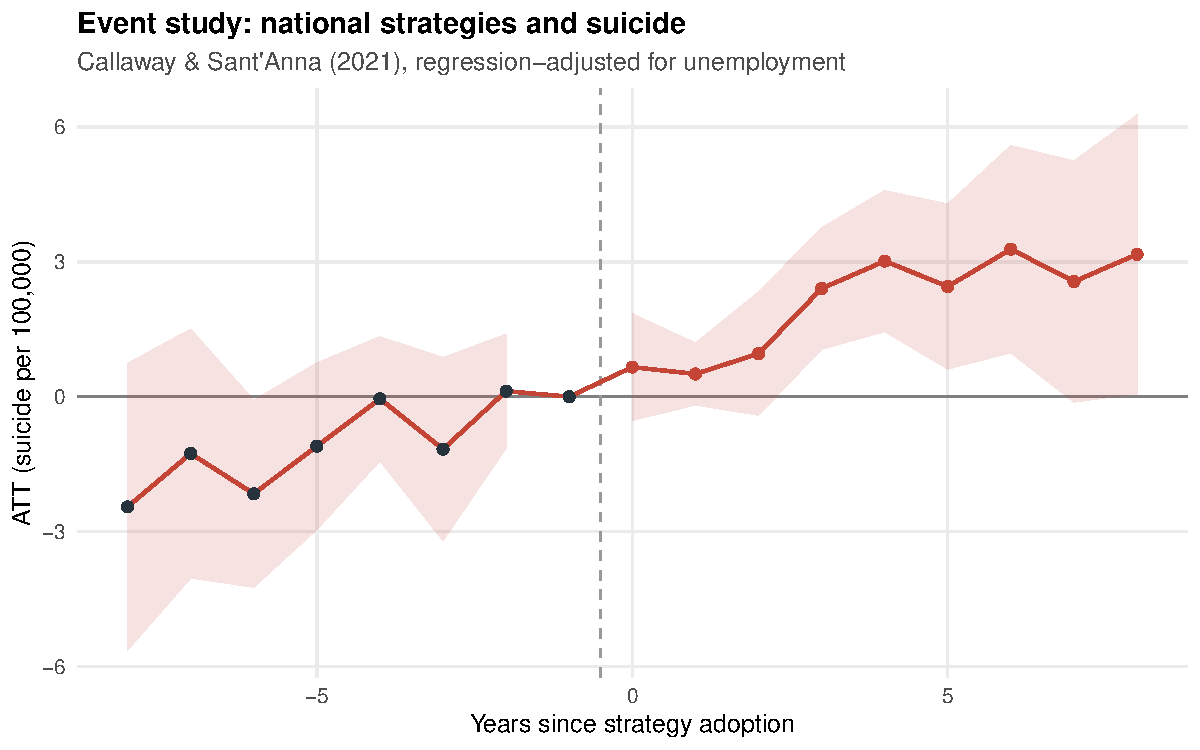
\includegraphics[height=0.70\textheight]{fig8_event_study.pdf}\\
{\color{warmgray}\small Long differences from $g\!-\!1$: $\sum z^2 = 9.9$ (8 d.f.) --- parallel trends not rejected.}
\end{frame}

\begin{frame}{A baseline can manufacture a pre-trend}
\vspace{0.4em}
\begin{columns}[T]
\begin{column}{0.48\textwidth}
\begin{alertblock}{Short differences (varying base)}
Each pre-coefficient is a one-period change.\\[0.4em]
$\sum z^2 = 59$ \;$\Rightarrow$\; ``trends fail.''
\end{alertblock}
\end{column}
\begin{column}{0.48\textwidth}
\begin{block}{Long differences (fixed $g\!-\!1$)}
Cumulative deviation from $g\!-\!1$ --- the same baseline as every post-coefficient, and as parallel trends itself.\\[0.4em]
$\sum z^2 = 9.9$ \;$\Rightarrow$\; flat.
\end{block}
\end{column}
\end{columns}
\vspace{0.5em}
\begin{center}\color{warmgray}The ``violation'' was an artifact of the wrong baseline. Most applied work reports the wrong one.\end{center}
\end{frame}

\begin{frame}{But flat is not a clean bill of health}
\vspace{0.8em}
The pre-trend leads are identified almost entirely off \textbf{the UK and Ireland}; Norway and Sweden (one pre-period each) feed the \emph{level} of the effect but not the \emph{test} of trends.\\[0.8em]
With four treated countries the test catches only gross violations.
\begin{center}\color{warmgray}It catches none --- the silence of a design too small to hear anything, not vindication.\end{center}
\end{frame}

\begin{frame}{The ``effect'' loads on the 2008 recession}
\centering
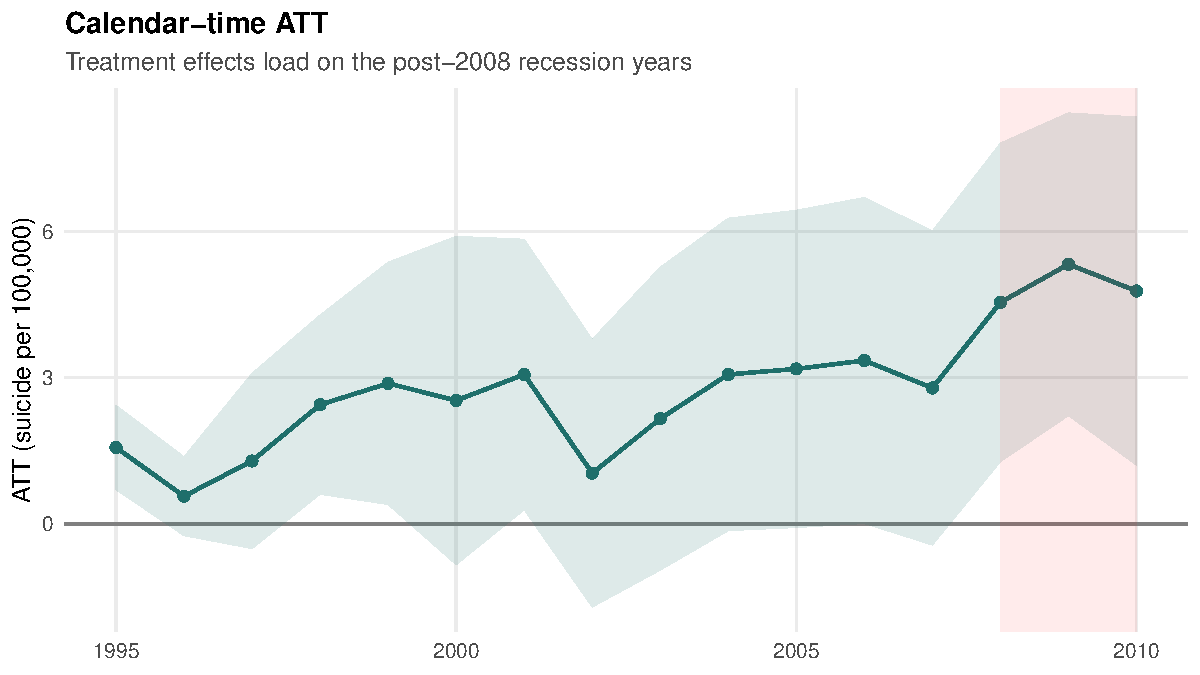
\includegraphics[height=0.70\textheight]{fig8c_calendar.pdf}\\
{\color{warmgray}\small The later cohorts' post-periods overlap Europe's austerity years.}
\end{frame}

\begin{frame}{The effect cannot be signed}
\centering
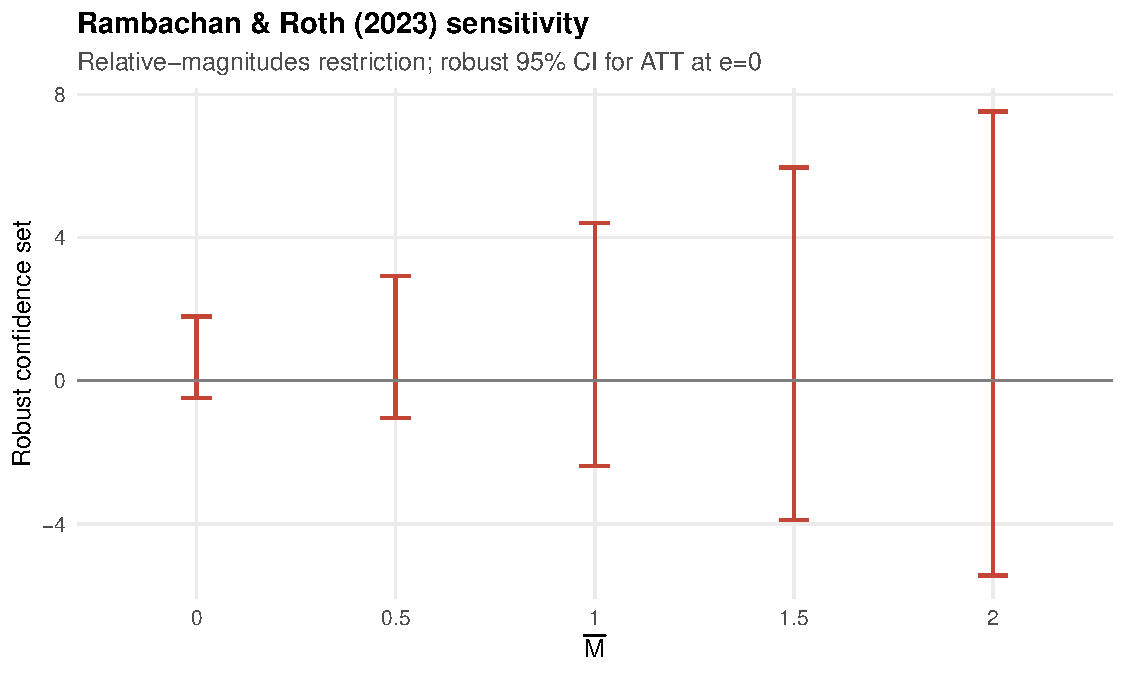
\includegraphics[height=0.66\textheight]{fig9_honestdid.pdf}\\
{\color{warmgray}\small Rambachan \& Roth (2023): under modest trend violations the robust CI spans zero.}
\end{frame}

\begin{frame}{Indistinguishable from chance}
\centering
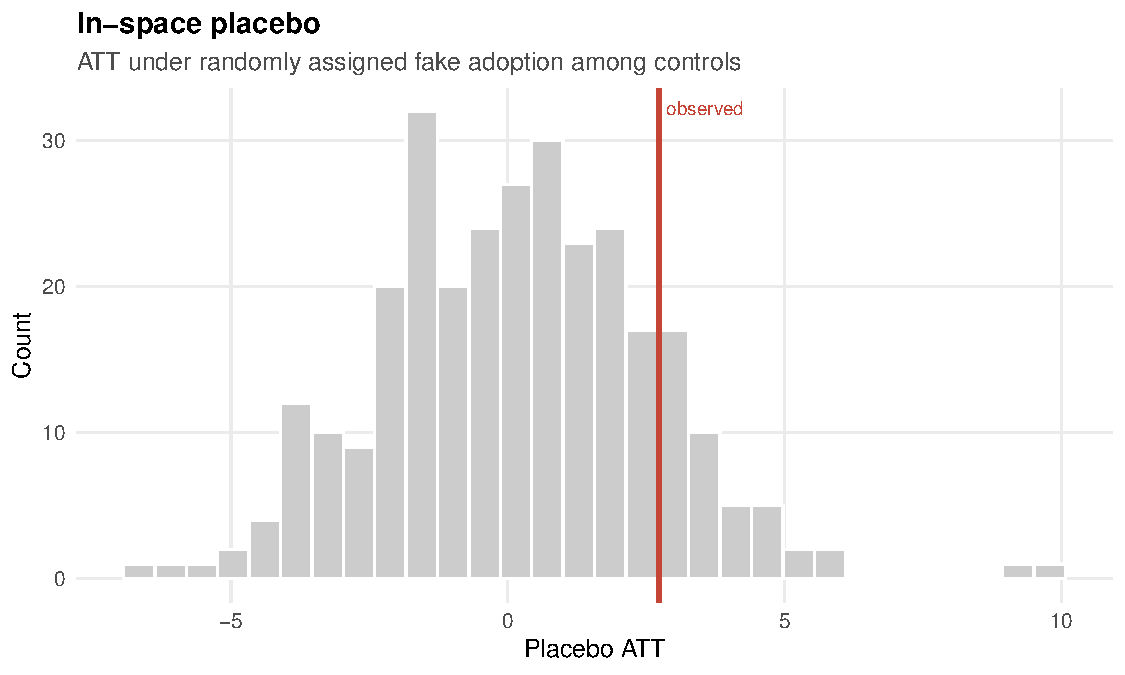
\includegraphics[height=0.66\textheight]{fig_falsification_placebo.pdf}\\
{\color{warmgray}\small One placebo in four, drawn from never-treated countries, is at least this large ($p=0.25$).}
\end{frame}

\begin{frame}{Even the method of last resort says nothing}
\begin{columns}[c]
\begin{column}{0.5\textwidth}
\centering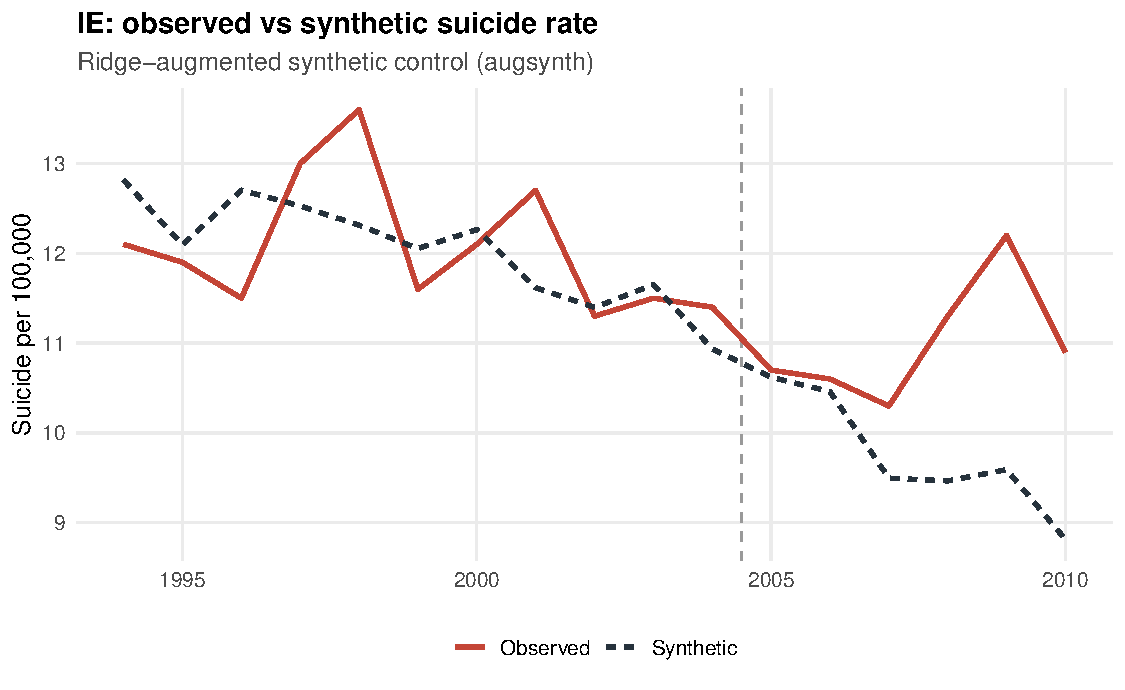
\includegraphics[width=\textwidth]{fig_synth_fit_IE.pdf}
\end{column}
\begin{column}{0.5\textwidth}
\centering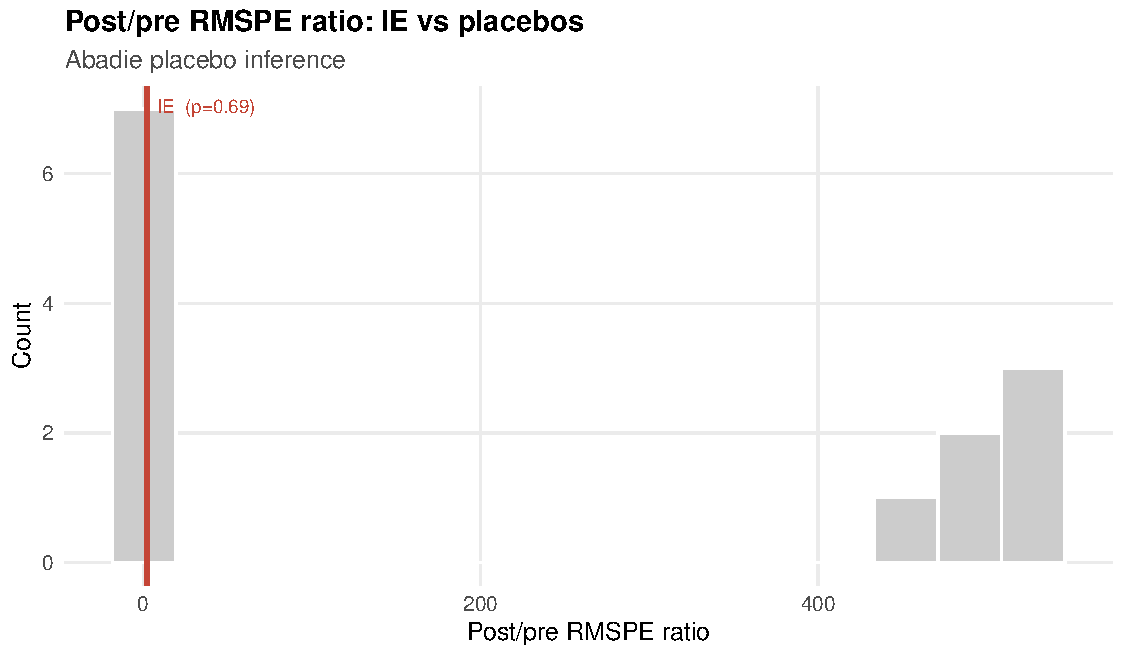
\includegraphics[width=\textwidth]{fig_synth_rmspe_IE.pdf}
\end{column}
\end{columns}
\begin{center}\color{warmgray}\small Augmented synthetic control: placebo $p=0.46$ (UK), $0.69$ (Ireland). Ireland's gap opens in 2008.\end{center}
\end{frame}

\begin{frame}{Fragile where a real effect would be solid}
\vfill
\begin{center}
{\Large Drop the four post-communist controls,}\\[0.4em]
{\Large and the estimate nearly halves: $+2.7 \;\rightarrow\; +1.2$.}
\end{center}
\vfill
\begin{center}\color{warmgray}A real treatment effect should not depend on which untreated countries you compare against. This one does.\end{center}
\vfill
\end{frame}

\begin{frame}{Is it just bad two-way fixed effects? No.}
\vspace{0.5em}
\centering
\begin{tabular}{lccc}
\toprule
Goodman-Bacon $2\times2$ & Weight & Est. & Contrib. \\
\midrule
\rowcolor{lightbg} Treated vs.\ untreated & 0.86 & 3.57 & 3.085 \\
Later vs.\ earlier treated & 0.11 & 0.29 & 0.032 \\
Earlier vs.\ later treated & 0.03 & $-0.22$ & $-0.005$ \\
\midrule
Reconstructed TWFE & 1.00 & & \textbf{3.11} \\
\bottomrule
\end{tabular}
\vspace{0.8em}
\begin{center}\color{warmgray}The ``forbidden'' comparisons carry $\sim$3\% weight. TWFE (3.11) $\approx$ CS (2.7). The estimator is not the problem --- identification is.\end{center}
\end{frame}

\divider{Devil's advocate}{The strongest objection}

\begin{frame}{``You are explaining away an inconvenient result''}
\vspace{0.6em}
\begin{block}{The skeptic}
You got a positive estimate and then argued it away with pre-trends and a recession. Convenient.
\end{block}
\vspace{0.4em}
\begin{alertblock}{The response}
I am \emph{not} claiming the recession explains the result --- that would identify, from a panel I called uninformative, an effect I have no business identifying. The claim is weaker and more durable: these forces are present, the design cannot separate them, and a number that confounds all three measures none.
\end{alertblock}
\end{frame}

\divider{What this means}{For the question, and for the Commission}

\begin{frame}{Not that strategies fail --- that we cannot see}
\vfill
\begin{center}
{\Large The finding is not that prevention is worthless.}\\[0.6em]
{\Large It is that the observational cross-section is \textbf{structurally incapable} of revealing its worth.}
\end{center}
\vfill
\begin{center}\color{warmgray}A policy can be both worth keeping and unproven. Honesty means holding both.\end{center}
\vfill
\end{frame}

\begin{frame}{We built a continent of strategies with no evaluation inside}
\vspace{0.8em}
No staggered randomization. No phased regional rollout with administrative mortality data. No pre-registered evaluation attached to a single national plan.\\[0.8em]
Every country switched at once, at the level where the confounders live, in response to the outcome itself.
\end{frame}

\begin{frame}{For the Commission: design the evaluation before the policy}
\begin{itemize}
\item Build the counterfactual \textbf{in}, not reconstruct it afterward.
\item Evaluate \textbf{below the nation} --- regions, phased rollout.
\item Pre-register the mortality outcome before deployment.
\end{itemize}
\vspace{0.5em}
\begin{center}\color{warmgray}The alternative is to keep spending moral and fiscal capital on faith.\end{center}
\end{frame}

\begin{frame}{Italy never wrote the document}
\vfill
\begin{center}
{\Large The country in which we sit is a documented \textbf{never-adopter}.}\\[0.6em]
{\large A large European nation that never wrote the strategy ---}\\[0.2em]
{\large the silent control against which the writers might have been judged,}\\[0.2em]
{\large had the data let us judge them.}
\end{center}
\vfill
\end{frame}

% ---------- Act III: closing ----------
\divider{We have been making life-and-death policy}{in a darkness we mistook for evidence.}

\end{document}
